\def\QRCODE{MASTER_mispa_TUT.IMG.gaussian_random_fields_matlabqrcode.png}
\def\QRPAGE{http://www.iptutorials.science/tree/master/MASTER_mispa/TUT.IMG.gaussian_random_fields/matlab}
\def\difficulty{3}
\mcorrectionsection{Matlab correction}

\subsection{White noise}
The white noise is generated with the following code. This is illustrated in Fig.\ref{fig:grf:matlab:wn}.
\begin{matlab}
%% white noise simulation
close all
n = 128;

W = randn(n);
imagesc(W);

imwrite_rf(W, 'wn.png');
\end{matlab}

In order to save a grayscale matrix as a colored image, the following code is necessary.
\begin{matlab}
function I = imwrite_rf(R, name)
% function that write a random field in a color image
%
% R: random field
% name: name of the image
%
% I: color image rgb

R = R - min(R(:));
R = 255 * R / max(R(:));
I = ind2rgb(uint8(R), jet(256));
imwrite(I, name);
\end{matlab}

\begin{figure}[htbp]
 \centering
 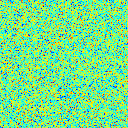
\includegraphics[width=5cm]{wn.png}
 \caption{White noise.}
 \label{fig:grf:matlab:wn}
\end{figure}

\subsection{Gaussian Random Field}
The Gaussian function that will serve as a covariance function is generated via the given code. Pay attention to the discretization grid: 
the FFT implies that functions are periodic, and in order to do that, the discretization must be set between $[-N/2:N/2[$.

\begin{matlab}
% gaussienne
N = 512;
N = 2^nextpow2(N); % force power of two
[Y, X] = meshgrid(-N/2:N/2-1, -N/2:N/2-1);

% covariance generation
sigma = 10;
Cmat = exp(-(X.^2+Y.^2)/(2*sigma^2));
figure()
h=surf(Cmat);
set(h, 'edgecolor','none')
\end{matlab}

The Gaussian Random Field can be generated via the formula already presented.
\begin{matlab}
% Fourier domain
% gaussian complex white noise
W=randn(N);

% covariance matrix in the Fourier domain
% ensure real values, although this is theoretically true
Cf = real(fft2(Cmat));

% ensure positive values, some numerical approximations can give negative values
Cf = sqrt(max(zeros(size(Cf)), Cf)); 

% phi_hat is the fourier transform of the gaussian random field
phi_hat = Cf.*fft2(W);

% we take the real part (should be real, but due to numerical
% approximations...)
G = real(ifft2(phi_hat));

% verify statistical properties
m = mean(G(:));
s = std(G(:));

figure()
imagesc(G);
imwrite_rf(G, 'grf.png');
\end{matlab}

\subsection{Minkowski functionals}

The Minkowski functionals are illustrated in Fig.\ref{fig:grf:matlab:Minkowski}. The code follows.

\begin{figure}[htbp]
 \centering
 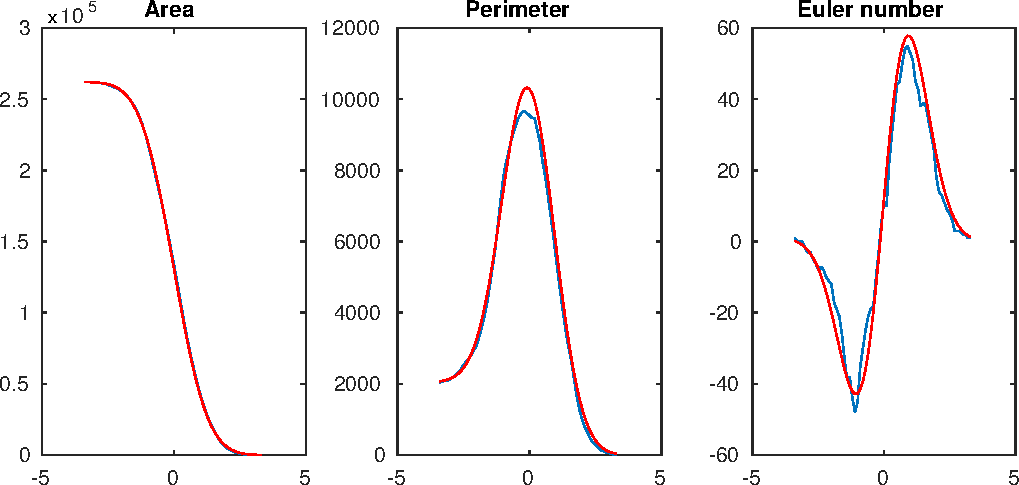
\includegraphics[width=\linewidth]{minko_levelset.pdf}
 \caption{Illustration of the simulated and analytical values of the Minkowski functionals of the level sets of the Gaussian Random Field.}
 \label{fig:grf:matlab:Minkowski}
\end{figure}

\begin{matlab}
% 
hmin = min(G(:));
hmax = max(G(:));
H = hmin:.1:hmax;

%
A = zeros(length(H), 1);
P = zeros(length(H), 1);
E = zeros(length(H), 1);

% analytical values
rho_0 = zeros(length(H), 1);
rho_1 = zeros(length(H), 1);
rho_2= zeros(length(H), 1);

lambda = 1/(2*sigma^2);

for i = 1:length(H)
    levelSet = G>=H(i);
    A(i) = bwarea(levelSet);
    P(i) = bwarea(bwperim(levelSet,4));
    E(i) = bweuler(levelSet,4);
    
    % analytic
    rho_0(i) =  1/2*erfc(H(i)/sqrt(2));
    rho_1(i) = sqrt(lambda)*exp(-H(i)^2/2)/(2*pi); 
    rho_2(i) = lambda /(2*pi)^(3/2) * exp(-(H(i)^2)/2)*H(i);
end
Aa = N^2*rho_0;
Pa = 4*N*rho_0 + pi*N^2*rho_1;
Ea = rho_0 + 2*N*rho_1 + N^2*rho_2;

%----------- display results
figure;
subplot(131);plot(H, A); hold on; 
plot(H, Aa, 'r'); title('Area');
subplot(132);plot(H, P); hold on; 
plot(H, Pa, 'r'); title('Perimeter');
subplot(133);plot(H, E); hold on; 
plot(H, Ea, 'r'); title('Euler number');
\end{matlab}